\chapter{Kiến trúc tổng thể của quy trình xây dựng đồ thị tri thức}

Chương này trình bày bức tranh tổng thể của quy trình xây dựng đồ thị tri thức từ dữ liệu văn bản tiếng Việt phi cấu trúc. Mục tiêu của chương không phải là mô tả chi tiết từng kỹ thuật xử lý, mà là làm rõ các khối chức năng chính, vai trò của từng khối và cách chúng nối tiếp nhau trong toàn bộ quy trình. Các bước cụ thể của từng thành phần sẽ được trình bày ở các chương sau.

Trong phạm vi khóa luận, dữ liệu đầu vào là các tài liệu công khai về Trường Đại học Công nghệ, Đại học Quốc gia Hà Nội. Các tài liệu này chứa thông tin về đơn vị, cán bộ, chương trình đào tạo, thông báo, sự kiện, văn bản và các hoạt động liên quan đến nhà trường. Đặc điểm chung của nguồn dữ liệu là thông tin phân tán ở nhiều bài viết, cùng một đối tượng có thể xuất hiện dưới nhiều cách gọi khác nhau, và nhiều quan hệ giữa các đối tượng không được biểu diễn sẵn dưới dạng có cấu trúc. Vì vậy, quy trình xây dựng đồ thị tri thức cần giải quyết ba vấn đề chính: trích xuất tri thức từ văn bản, hợp nhất các thực thể trùng lặp và kiểm soát các trường hợp không đủ chắc chắn bằng sự can thiệp của con người (human fallback).

\begin{figure}[H]
    \centering
    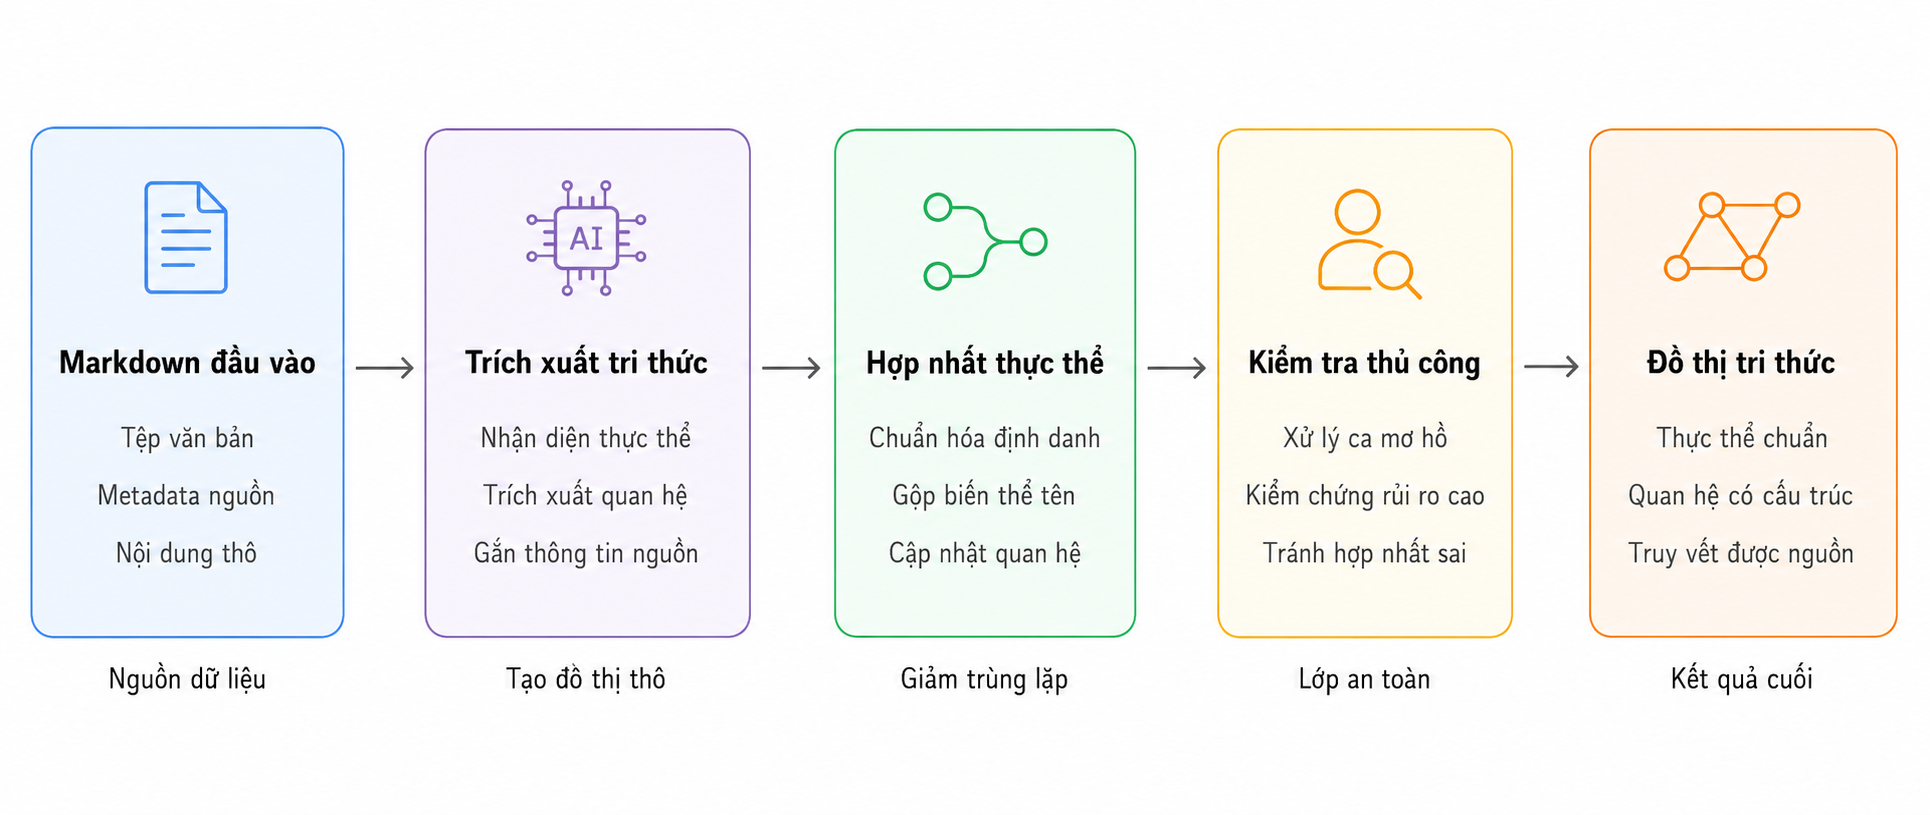
\includegraphics[width=\textwidth]{image/generated/chapter3/architecture-overview.png}
    \caption{Kiến trúc tổng thể của quy trình xây dựng đồ thị tri thức}
    \label{fig:architecture-overview}
\end{figure}

Hình~\ref{fig:architecture-overview} mô tả quy trình ở mức tổng quan thông qua năm khối chính. Khối dữ liệu tiếp nhận các tài liệu văn bản đã được xử lý và gắn thông tin nguồn. Từ dữ liệu này, hệ thống thực hiện trích xuất tri thức để nhận diện thực thể, quan hệ và bằng chứng văn bản tương ứng. Kết quả sau trích xuất vẫn là các mảnh tri thức ban đầu, nên cần được đưa sang bước xử lý đồng tham chiếu để phát hiện các biến thể tên gọi và hợp nhất các thực thể cùng tham chiếu đến một đối tượng.

Sau bước xử lý đồng tham chiếu, các trường hợp mơ hồ hoặc có rủi ro hợp nhất sai được chuyển sang human fallback để con người kiểm chứng trước khi chấp nhận quyết định cuối cùng. Kết quả của toàn bộ quy trình là một đồ thị tri thức có cấu trúc, trong đó thực thể và quan hệ được tổ chức nhất quán hơn và vẫn có thể truy vết về nguồn văn bản ban đầu thông qua \texttt{chunk\_id}, metadata và bằng chứng đi kèm. Các chi tiết kỹ thuật của từng khối, như gom nhóm chunks, thiết kế prompt, chuẩn hóa thực thể, embedding và tìm kiếm ứng viên đồng tham chiếu, được trình bày ở các chương tiếp theo.

\begin{figure}[H]
    \centering
    \makebox[\textwidth][c]{%
        \begin{minipage}[t]{0.54\textwidth}
            \centering
            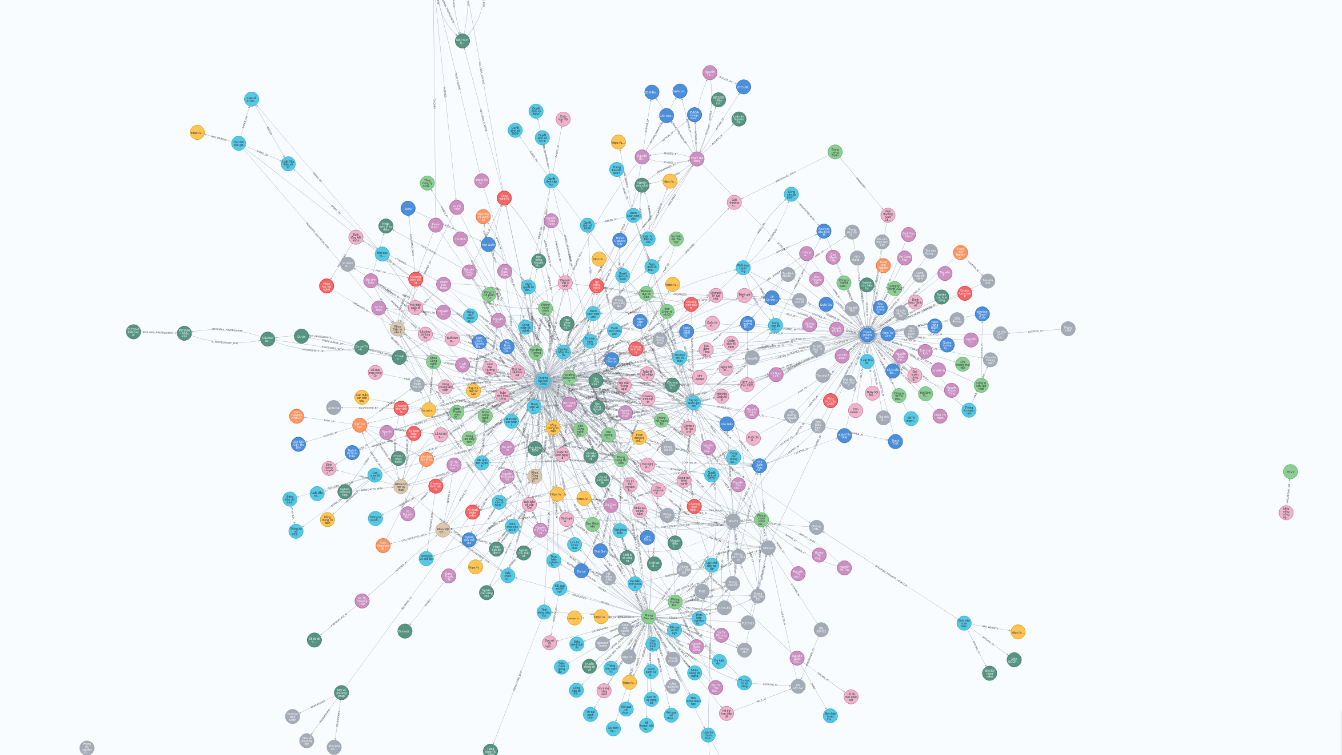
\includegraphics[width=\linewidth]{image/static/raw_graph_visualize.png}
            \vspace{2pt}
            {\small (a) Đồ thị thô sau trích xuất}
        \end{minipage}%
        \hspace{0.02\textwidth}%
        \begin{minipage}[t]{0.54\textwidth}
            \centering
            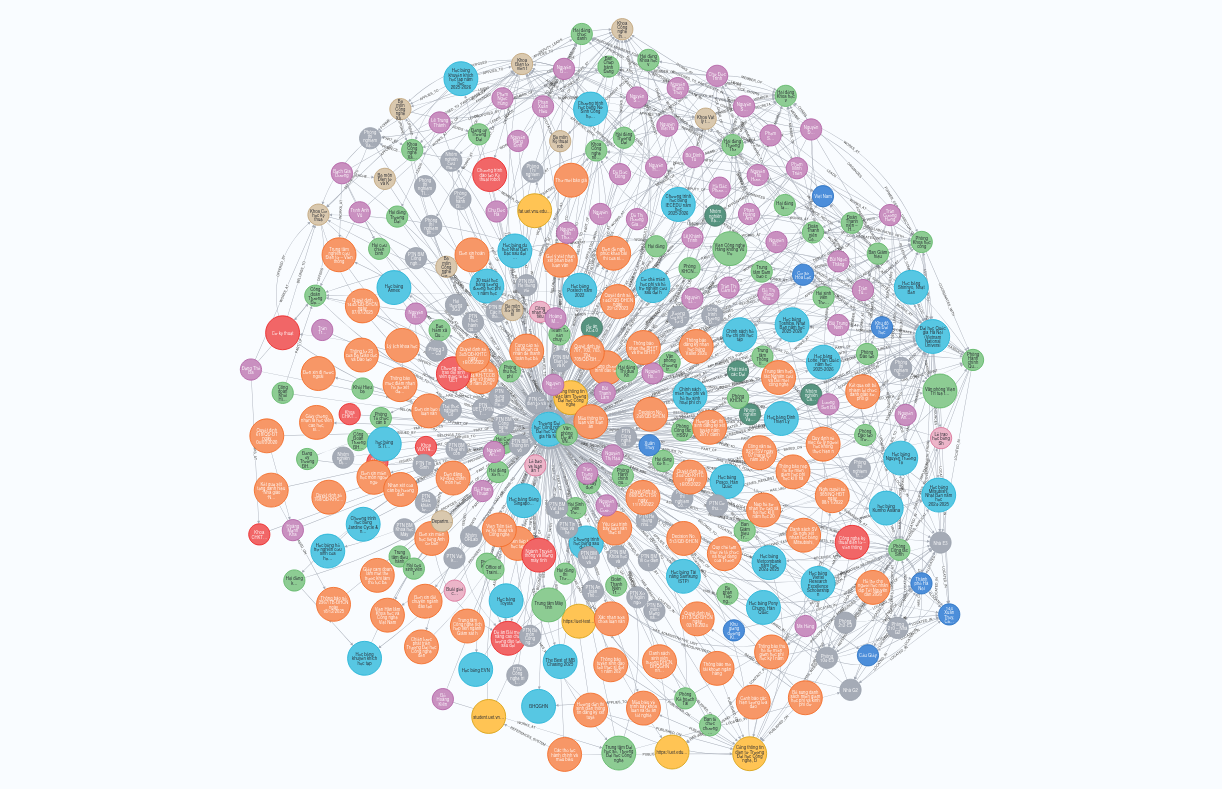
\includegraphics[width=\linewidth]{image/static/graph_visualize.png}
            \vspace{2pt}
            {\small (b) Đồ thị sau tổ chức và hợp nhất}
        \end{minipage}%
    }
    \vspace{6pt}

    \makebox[\textwidth][c]{%
        \begin{minipage}[t]{1.08\textwidth}
            \centering
            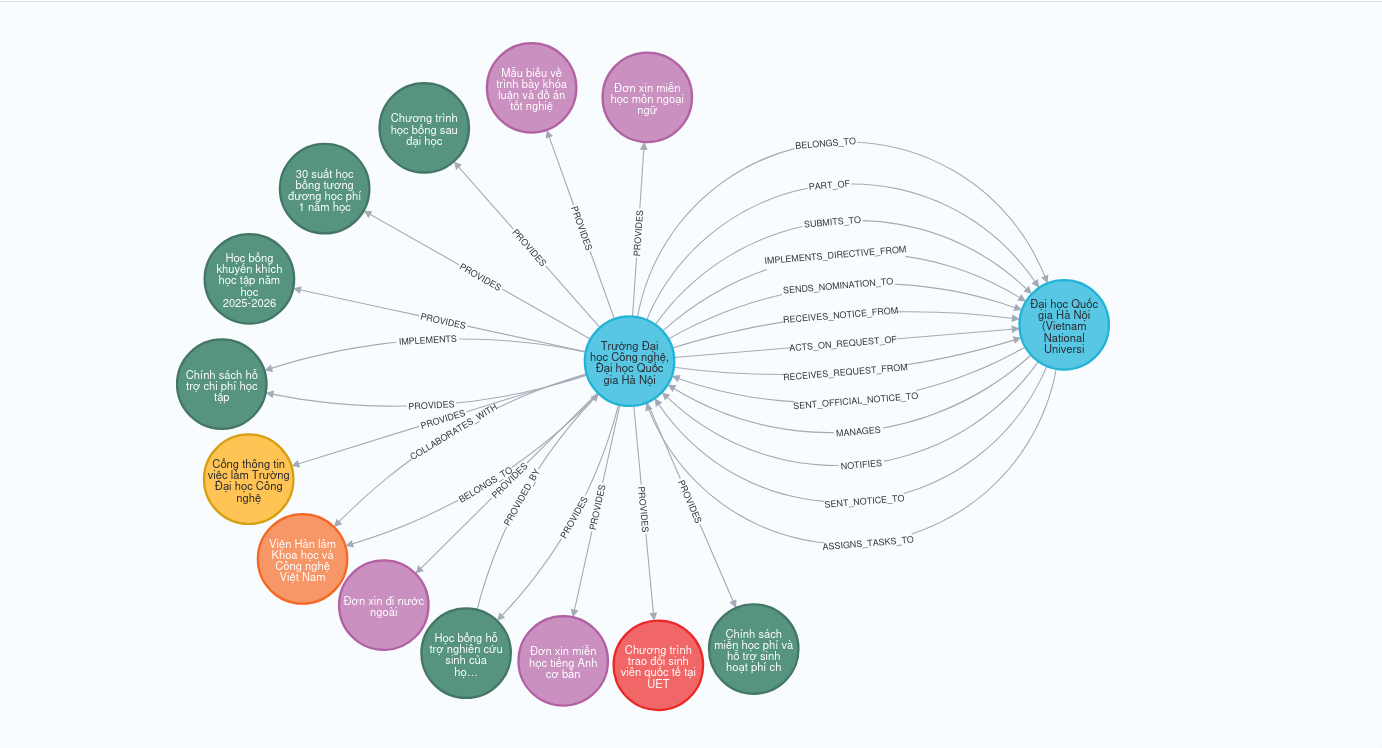
\includegraphics[width=\linewidth]{image/static/mini_graph_visualize.png}
            \vspace{2pt}
            {\small (c) Minh họa với 15 thực thể}
        \end{minipage}%
    }
    \caption{So sánh đồ thị tri thức trước và sau khi tổ chức các thực thể và quan hệ}
    \label{fig:graph-visualize}
\end{figure}

Hình~\ref{fig:graph-visualize} minh họa sự thay đổi của đồ thị tri thức trong quy trình xử lý. Ở bên trái, đồ thị thô sau trích xuất còn phân tán và chứa nhiều cụm rời rạc do các thực thể được tạo từ từng tài liệu hoặc từng phân đoạn riêng lẻ. Ở bên phải, sau khi tổ chức lại thực thể, hợp nhất các trường hợp đồng tham chiếu và cập nhật quan hệ, đồ thị trở nên tập trung hơn, giúp quan sát rõ hơn các liên kết giữa các đối tượng và tạo nền tảng tốt hơn cho phần đánh giá hỏi đáp ở Chương~6.

Từ kiến trúc tổng thể này, các chương tiếp theo đi vào từng phần của quy trình. Chương 4 trình bày quy trình trích xuất tri thức từ dữ liệu. Chương 5 trình bày xử lý đồng tham chiếu thực thể và cơ chế human fallback. Chương 6 trình bày thực nghiệm và đánh giá, trong đó phần hỏi đáp được dùng để kiểm tra giá trị sử dụng của đồ thị tri thức ở lớp ứng dụng.
